\documentclass[journal,onecolumn]{IEEEtran}

\usepackage{amsmath,amssymb,amsfonts}
\usepackage{graphicx}
\graphicspath{{../results/figures/}{figures/}{./}}
\usepackage{booktabs}
\usepackage{cite}
\usepackage{hyperref}
\usepackage{url}

% Supplementary items are numbered S1, S2, ... so they cannot be confused with the main text.
\renewcommand{\thetable}{S\arabic{table}}
\renewcommand{\thefigure}{S\arabic{figure}}
\renewcommand{\thesection}{S\arabic{section}}

\begin{document}

\title{Supplementary Material for ``OmniST: Topology-Invariant Forecasting for Dynamic Sensor
Networks With Guaranteed Coverage at Unseen Sensors''}
\author{Praveg~Vashishtha}
\maketitle

This document collects results that support the main paper but did not fit its page budget. Every
number here comes from the same committed result files as the main text and reproduces from the
released scripts at \url{https://github.com/Praveg432/OmniST}.

\section{Month-by-Month Accuracy Against Published E-STGCN Numbers}

Table~\ref{tab:monthly} lists 30-day PM$_{2.5}$ MAE for each month of 2023 on the Delhi CPCB data,
next to the values published for E-STGCN~\cite{panja2026estgcn} on the same split. The OmniST values
come from a single representative run, kept for month-level readability; the seed-hardened figure in
the main text is the 5-seed MAE of $28.2\pm0.9$~$\mu$g/m$^3$. Because the E-STGCN numbers are
published values under a protocol we did not run, the controlled reimplementation in the main paper
is the comparison we rely on.

\begin{table}[htbp]
\caption{30-Day PM$_{2.5}$ MAE ($\mu$g/m$^3$) on Delhi CPCB Data (2023), Single Run}
\centering
\begin{tabular}{lccl}
\toprule
\textbf{Month} & \textbf{OmniST} & \textbf{E-STGCN}$^*$ & \textbf{Note} \\
\midrule
Jan & 57.3 & 56.1 & Comparable \\
Mar & 24.2 & 25.8 & Comparable \\
Apr & 22.0 & 25.4 & OmniST better \\
May & 30.9 & 29.0 & Comparable \\
Jun & 18.1 & 22.0 & OmniST better \\
Jul & 11.3 & 15.7 & OmniST better \\
Aug & 11.2 & 11.9 & Comparable \\
Sep & 15.2 & 15.1 & Comparable \\
Oct & 30.4 & 36.4 & OmniST better \\
Nov & 69.8 & 77.1 & OmniST better \\
Dec & 50.9 & 116.8$^\dagger$ & See note \\
\midrule
Avg & 31.0 & 39.2 & \\
\bottomrule
\multicolumn{4}{l}{\footnotesize $^*$From E-STGCN Table 2~\cite{panja2026estgcn}; direct comparison requires caution.} \\
\multicolumn{4}{l}{\footnotesize $^\dagger$Exceeds naive baselines; a methodological difference is likely.} \\
\end{tabular}
\label{tab:monthly}
\end{table}

In the moderate-pollution months (April to September) the two methods are within
3~$\mu$g/m$^3$ of each other. In December the published E-STGCN MAE (116.8) exceeds even a naive
``predict the recent average'' baseline (48.9~$\mu$g/m$^3$). We cannot tell whether that reflects a
methodological difference or a real failure mode without running the authors' code, so we make no
claim of winter superiority.

\section{Ablation of the Spatial Component}

Table~\ref{tab:ablation} ablates the spatial attention and the neighbourhood size on coverage and
inductive MAE at unseen nodes. Removing the attention entirely (coordinate MLP plus temporal backbone
only) or changing $k$ moves coverage by at most about $0.01$ on every domain. The coverage guarantee
is therefore earned by the coordinate-based inductive construction, which lets each node be scored
from its own coordinates and local context, rather than by the attention layer or a particular $k$.
The attention's role is to make inductive prediction possible and to sharpen intervals slightly.

\begin{table}[htbp]
\caption{Ablation: Coverage and Inductive MAE at Unseen Nodes (Target 90\%)}
\centering
\begin{tabular}{llccc}
\toprule
\textbf{Dataset} & \textbf{Metric} & \textbf{Full} & \textbf{No GAT} & \textbf{$k{=}4$ / $k{=}16$} \\
\midrule
Delhi AQ   & coverage & 0.915 & 0.912 & 0.914 / 0.913 \\
           & ind-MAE  & 26.7  & 26.4  & 26.2 / 26.1 \\
Weather    & coverage & 0.917 & 0.925 & 0.920 / 0.922 \\
           & ind-MAE  & 4.99  & 4.80  & 4.92 / 4.97 \\
Traffic    & coverage & 0.919 & 0.919 & 0.919 / 0.919 \\
           & ind-MAE  & 9.55  & 9.54  & 9.63 / 9.63 \\
\bottomrule
\end{tabular}
\label{tab:ablation}
\end{table}

\section{Calibration Diagnostics and Multiple Coverage Targets}

Fig.~\ref{fig:calibration} plots empirical against target coverage for
$\alpha\in\{0.5,\dots,0.95\}$ on each dataset; every curve tracks the diagonal. A split by residual
tercile shows near-complete coverage on the low and middle strata and lower coverage on the highest
stratum ($\approx0.73$--$0.78$). Because the strata are defined by residual size, the high stratum is
partly hard by construction; we report it as a limit of marginal coverage rather than a separate
failure.

Repeating the inductive evaluation at targets of 80, 90 and 95\% (5 seeds for air quality, 3 for
traffic) gives empirical coverage within about 3 points of the target in every cell: Delhi
$0.824/0.915/0.958$, Beijing $0.801/0.928/0.968$, and traffic $0.773/0.911/0.963$. The loosest cell
is traffic at the 80\% target ($0.773$).

\begin{figure}[htbp]
\centering
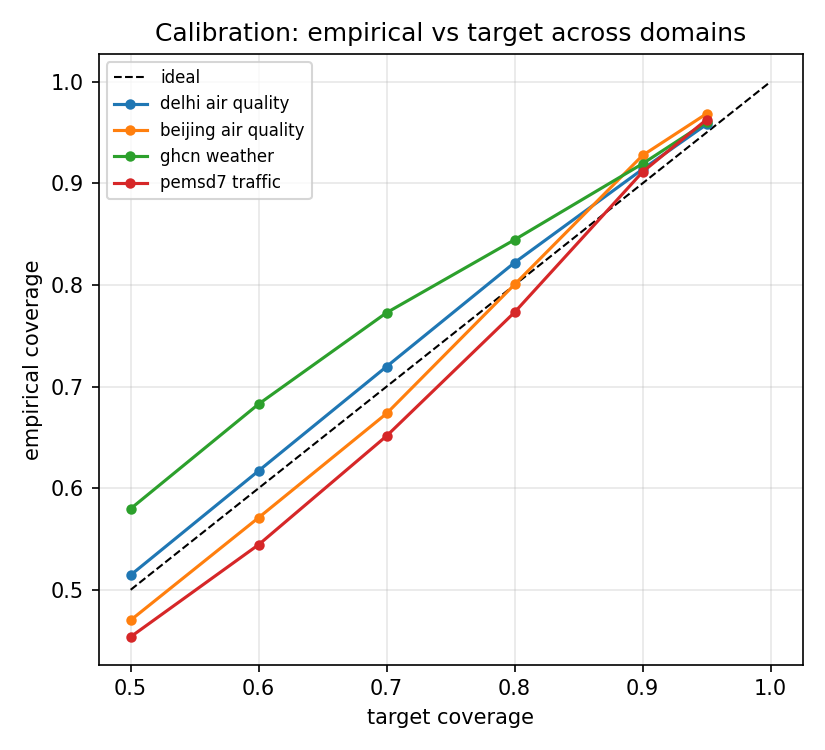
\includegraphics[width=0.6\columnwidth]{fig_calibration.png}
\caption{Calibration curves (empirical against target coverage) across the four real datasets.}
\label{fig:calibration}
\end{figure}

\section{Conditional Coverage and Mondrian Conformal}

The guarantee is marginal. Per-unseen-node coverage at the 90\% target is close to conditional on the
air-quality networks (spread $0.87$--$0.95$) but not on the irregular traffic network (spread
$0.73$--$0.98$, averaging a valid $0.92$). Grouping unseen nodes by distance to the nearest training
node and calibrating a separate quantile per group (Mondrian conformal) lifts the worst-group coverage
on traffic from $0.80$ to $0.86$, giving that group a wider interval ($51.5$ against $42.1$), and
leaves the air-quality domains unchanged (Fig.~\ref{fig:mondrian}). This narrows the gap without
closing it ($0.86 < 0.90$).

\begin{figure}[htbp]
\centering
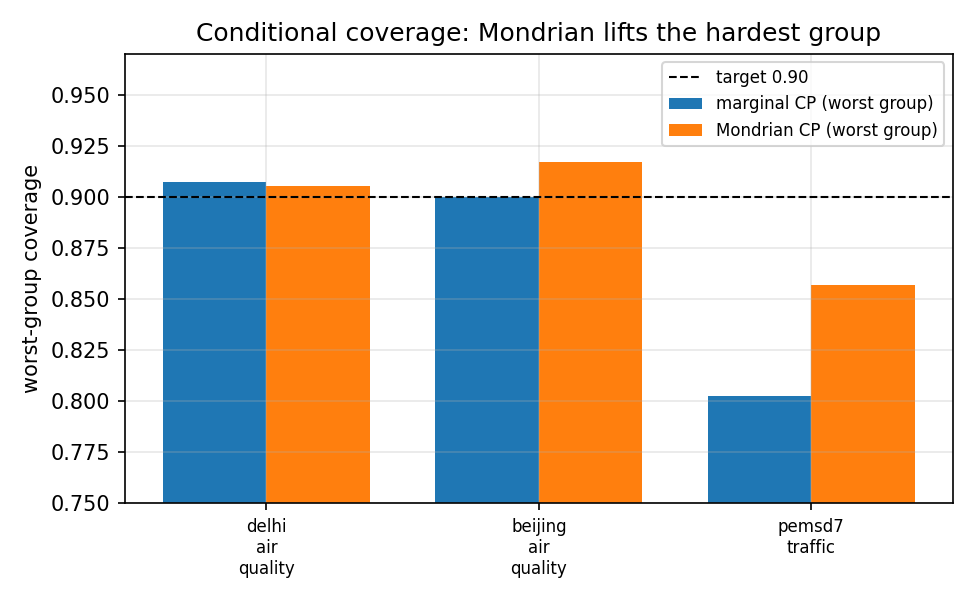
\includegraphics[width=0.6\columnwidth]{fig_mondrian.png}
\caption{Mondrian conformal lifts the worst-group coverage on the traffic network from 0.80 toward
the target and leaves the air-quality domains unchanged.}
\label{fig:mondrian}
\end{figure}

\section{Computational Scaling}

A cost stress test that replicates real sensors with coordinate jitter shows training time growing
super-linearly ($169\to437\to1106$\,s for $228\to456\to912$ nodes), the signature of exact $O(N^2)$
$k$-NN attention. This test does not certify coverage, because duplicating nodes breaks calibration
exchangeability. A scalable variant (a cKDTree neighbour index with an index-select gather) is
numerically equivalent to exact attention (output cosine similarity $0.99996$ at $N{=}228$) and
$2.3\times$ faster per forward pass at $N{=}1824$, with the gap widening in $N$.

\bibliographystyle{IEEEtran}
\bibliography{references}

\end{document}
